%++++++++++++++++++++++++++++++++++++++++
% Don't modify this section unless you know what you're doing!
\documentclass[letterpaper,12pt]{article}
\usepackage{tabularx} % extra features for tabular environment
\usepackage{amsmath,amsthm,amssymb,amsfonts}  % improve math presentation
\usepackage{graphicx} % takes care of graphic including machinery
\usepackage[margin=1in,letterpaper]{geometry} % decreases margins
\usepackage{cite} % takes care of citations
\usepackage[final]{hyperref} % adds hyper links inside the generated pdf file
\hypersetup{
	colorlinks=true,       % false: boxed links; true: colored links
	linkcolor=blue,        % color of internal links
	citecolor=blue,        % color of links to bibliography
	filecolor=magenta,     % color of file links
	urlcolor=blue         
}
%++++++++++++++++++++++++++++++++++++++++


%Blackboard Letters

\newcommand{\R}{\ensuremath{\mathbb{R}}}
\newcommand{\C}{\ensuremath{\mathbb{C}}}
\newcommand{\Z}{\ensuremath{\mathbb{Z}}}
\newcommand{\Q}{\mathbb{Q}}
\newcommand{\N}{\mathbb{N}}
\newcommand{\F}{\mathbb{F}}
\newcommand{\W}{\mathbb{W}}
\newcommand{\Prob}{\mathbb{P}}
\newcommand{\E}{\mathbb{E}}

%Differential d
\newcommand*{\diff}{\mathop{}\!\mathrm{d}}

% Theorem / Lemmas et cetera

\newtheorem{thm}{Theorem}[section]
\newtheorem{conj}[thm]{Conjecture}
\newtheorem{cor}[thm]{Corollary}
\newtheorem{lem}[thm]{Lemma}
\newtheorem{prop}[thm]{Proposition}
\newtheorem{exa}[thm]{Example}
\newtheorem{defi}[thm]{Definition}
\newtheorem{exe}[thm]{Exercise}
\newtheorem{rek}[thm]{Remark}
\newtheorem{que}[thm]{Question}
\newtheorem{prob}[thm]{Problem}
\newtheorem{cla}[thm]{Claim}

\begin{document}

\title{C1 Assignment 4 Report}
\author{1104630}
\date{\today}
\maketitle


\section{Question 1: Monte Carlo Methods}

\subsection{Theory}

We wish to solve
\[
I = \int_{[ 0 , 1 ] ^N} f(x) \diff x
\]
for some $f : \R^N \to \R$.

Monte Carlo integration involves using randomness to solve deterministic problems allowing us to obtain better convergence results for higher dimensional integrals than would be otherwise possible if deterministic methods were used. To do this we consider a sequence of independent, identically distributed random vectors $X_i : \Omega \to \R^N$ where $i \in \N$ and define an unbiased estimator $F_n$ by
\[
F_n = \frac{1}{M} \sum_{i = 1}^{M} f(X_i).
\]
where $M$ is the number of sampled used. We note that
\begin{align*}
\E[F_N] = \frac{1}{N} \sum_{i = 1}^{M} \E [f(X_i)] = \E[f(X_1)] = \int_{\R^N} f(x)p(x) \diff x = I
\end{align*}
where $p$ is the distribution of $X_1$. In particular, by choosing $X_i$ to be uniform random variables on $[0 , 1]^N$ we find that $\E[F_n] = I$. 

We know from the Strong Law of Large Numbers that $F_n \to I \text{ a.s.}$ as $n \to \infty$. We are also interested in the error between the value of the integral and its Monte Carlo estimation. By the Central Limit theorem, we know that
\[
F_n \to \mathcal{N}(I , \frac{\sigma^2}{n} )
\]
in distribution as $n \to \infty$ where $\text{Var}(f(X_1)) = \sigma^2$. Therefore the error of $F_n$ is approximately $\frac{\sigma}{\sqrt{n}}$. We note that this error estimate is independent of the dimension $N$.

\subsection{Results}

We obtain the following results:

\centerline{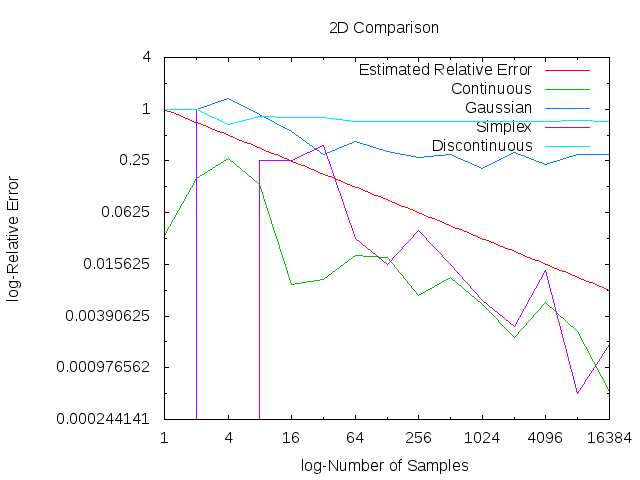
\includegraphics[scale = 0.8]{/home/john/Dropbox/C1/Assignment_4/Q1/2D.png}}

\centerline{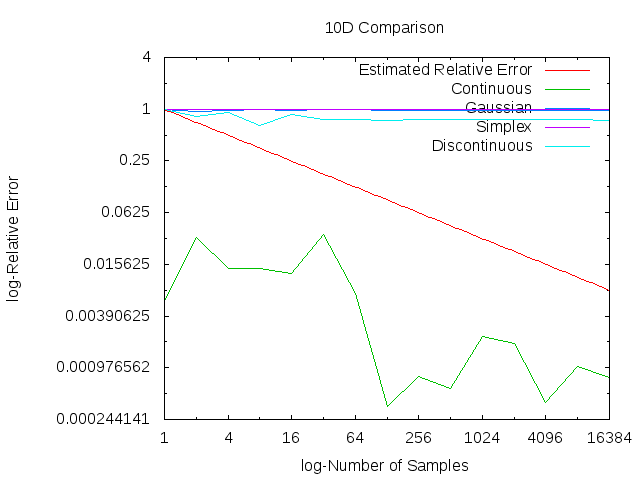
\includegraphics[scale = 0.8]{/home/john/Dropbox/C1/Assignment_4/Q1/10D.png}}

From the graphs we see that error of all the models is erratic when compared with $\frac{1}{\sqrt{n}}$ due to the randomness of the Monte Carlo simulation. Furthermore, we note that in both 2 dimensions and 10 dimensions only the Continuous model has smaller relative error than $\frac{1}{\sqrt{n}}$ while the Gaussian, Simplex and Discontinuous models have larger relative errors.


\section{Question 2: ODEs with Uncertain Parameters}

\subsection{Theory}

In this question we numerically solve the IVP from assignment 3 with a random parameter using Monte Carlo methods. 

\subsection{Results}

\subsubsection{Expectations and Variances}

We obtain the ollowing graphs:

\centerline{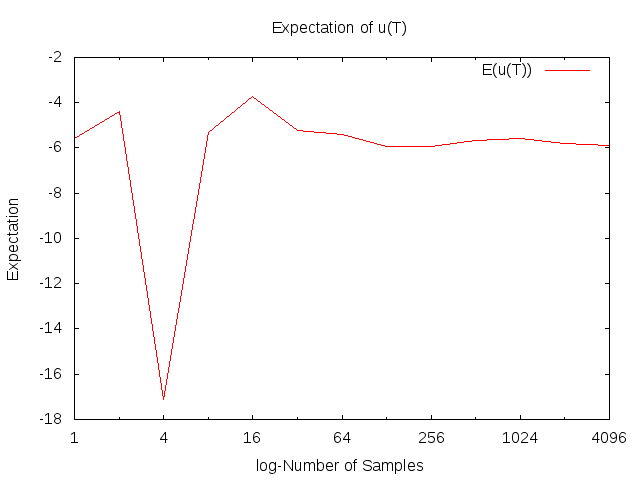
\includegraphics[scale = 0.4]{/home/john/Dropbox/C1/Assignment_4/Q2/expectation_u.png}}

\centerline{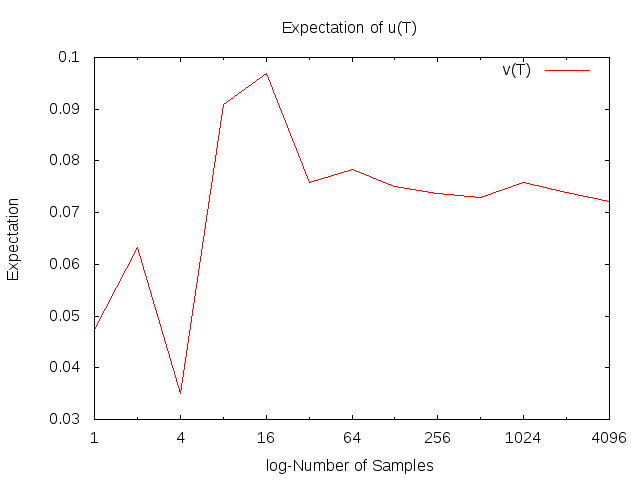
\includegraphics[scale = 0.4]{/home/john/Dropbox/C1/Assignment_4/Q2/expectation_v.png}}


\centerline{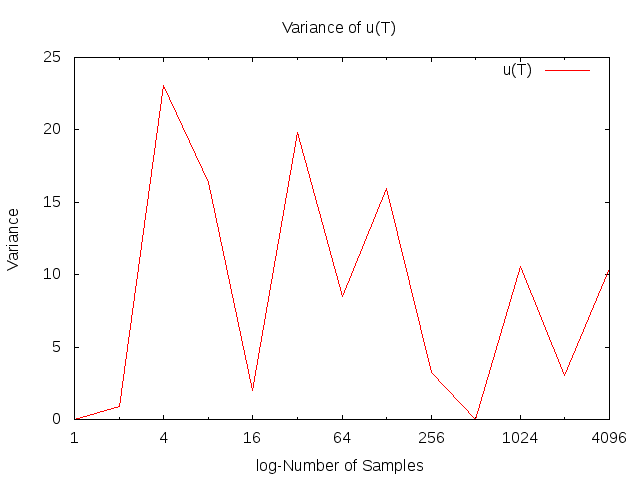
\includegraphics[scale = 0.4]{/home/john/Dropbox/C1/Assignment_4/Q2/variance_u.png}}


\centerline{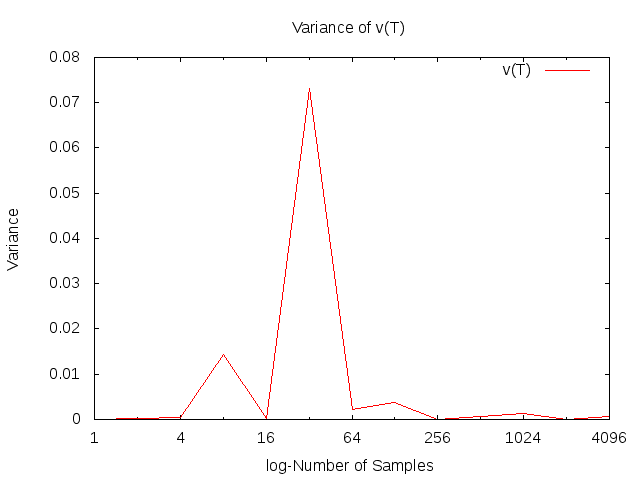
\includegraphics[scale = 0.4]{/home/john/Dropbox/C1/Assignment_4/Q2/variance_v.png}}

From the graphs we note that the means appear to be converging while the variances have no descernable pattern. This is possibly due to the approximation error from calculating the mean which is used to caluclate the variance.


\subsubsection{Histogram of $v(T)$ }

\centerline{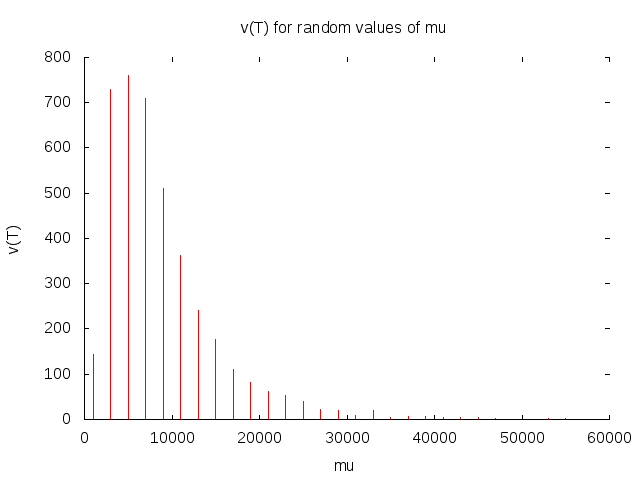
\includegraphics[scale = 0.8]{/home/john/Dropbox/C1/Assignment_4/Q2/histogram.png}}

From the graph, the distribution of various samples of $v(T)$ appear to be lognormally distributed. By considering the exact solution of $v(T) = \frac{\mu}{\lambda + T^3 - T^2}$ which is lognormally distributed as $\mu$ is lognormally distributed.



\section{Question 3: Advection-Diffusion Equation}

\subsection{Theory}

We are interested in solving the following boundary value problem numerically:

\[
-\alpha \frac{\diff^2 u}{\diff x^2 } + \beta \frac{\diff u}{\diff x } = 0
\]
on the interval $[0, L]$ with $u(0) = 0$ and $u(L) = 1$ and $\alpha > 0$ and $\beta > 0$ are given constants. This equation has solution
\[
u(x) = \frac{e^{\frac{\beta x}{\alpha}} - 1}{e^{\frac{\beta L}{\alpha}} - 1}.
\]
We model the differential equation using a finite difference approximation. We first divide the interval $[0 , L]$ into $N$ uniformly spaced grid points and then we obtain the following approximation:
\[
\frac{\alpha}{h^2}(u_{i - 1} + 2u_i + u_{i + 1}) + \frac{\beta}{h}(u_{i + 1} - u_{i - 1} ) = 0
\]
for $i = 1, \cdots, N -1$ with $u_0 = 0$ and $u_N = 1$ as boundary conditions. By solving this difference equation, we find the solution for $u_i$ to be
\[
u_i = \Bigg( 1 - \Big(\frac{1 + \Prob e}{1-\Prob e} \Big)^i \Bigg) /\Bigg( 1 - \Big(\frac{1 + \Prob e}{1-\Prob e} \Big)^n \Bigg)
\]
where $\Prob e = \frac{\beta h}{\alpha}$ is the local P\'{e}clet number where $h$ is the step size.

\subsection{Results}

Throughout, we fix $L = 1$ and $N = 100$.

\subsubsection{ $\Prob e_{gl} \approx 0$ }

For this test, we took $\alpha = 1.0$ and  $\beta = 1.0 \times 10^{-9}$ and obtained the following results.

\centerline{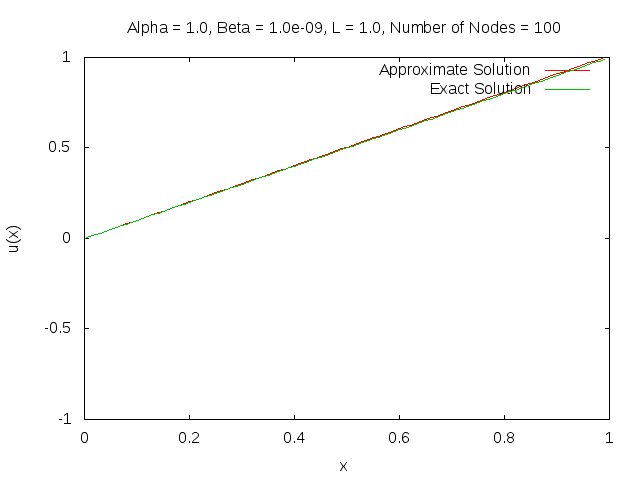
\includegraphics[scale = 0.5]{/home/john/Dropbox/C1/Assignment_4/Q3/1_1e-09_1_100.png}}

\centerline{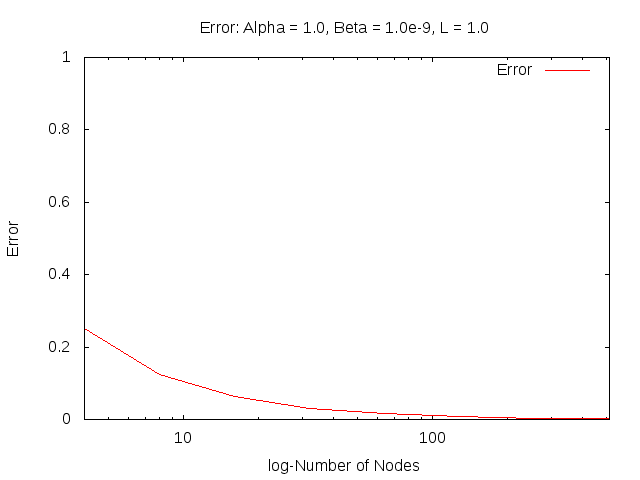
\includegraphics[scale = 0.5]{/home/john/Dropbox/C1/Assignment_4/Q3/Error_Plot_1_1e-09_1.png}}

When $\beta$ is made very small the advection term becomes negligible and the BVP becomes close to its limit problem $-u'' = 0$ which has linear solution. From the first graph, we see that the finite difference approximation is very effective in this case with the error decreasing rapidly as the number of samples increases.



\subsubsection{ $\Prob e_{gl} = 1$ }

For this test, we took $\alpha = 1.0$ and  $\beta = 2.0$ and obtained the following results.


\centerline{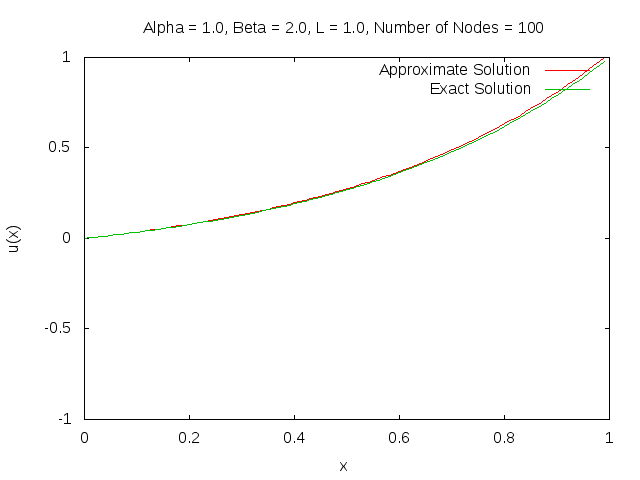
\includegraphics[scale = 0.5]{/home/john/Dropbox/C1/Assignment_4/Q3/1_2_1_100.png}}

\centerline{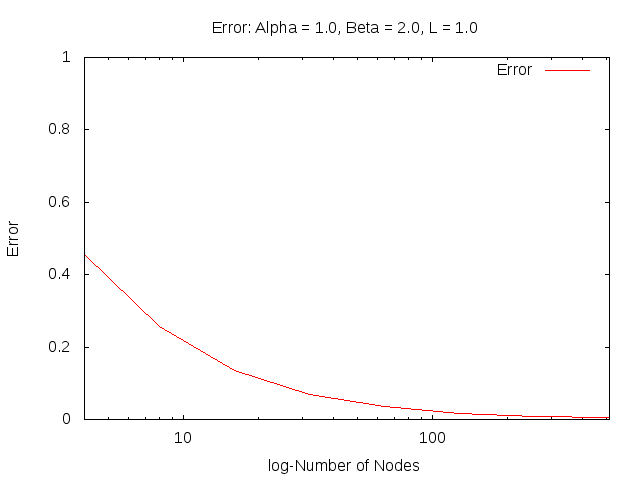
\includegraphics[scale = 0.5]{/home/john/Dropbox/C1/Assignment_4/Q3/Error_Plot_1_2_1.png}}

With the P\'{e}clet number near unity, the advection term becomes non-negligible and both the approximate and exact solutions are no longer linear. In particular, by comparing the error between the case where $\Prob e_{gl} \approx 0$ and $\Prob e_{gl} = 1$, we can see that the finite difference approximation in the latter case creates a larger error than the former.  


\subsubsection{ $\Prob e_{gl} >> 1$ }


For this test, we took $\alpha = 1.0$ and  $\beta = 1000.0$ and obtained the following results.


\centerline{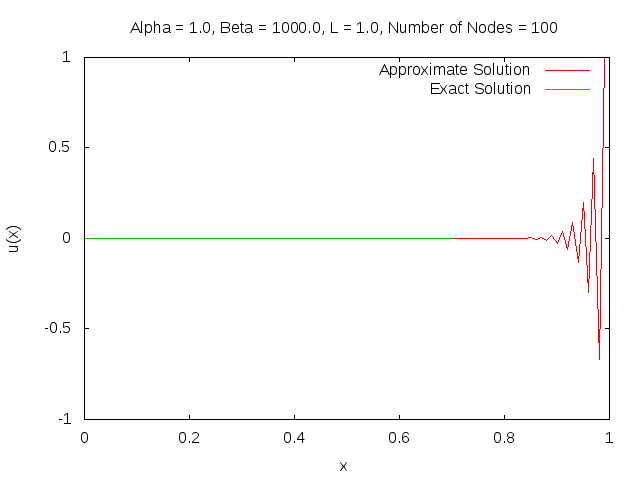
\includegraphics[scale = 0.5]{/home/john/Dropbox/C1/Assignment_4/Q3/1_1000_1_100.png}}

\centerline{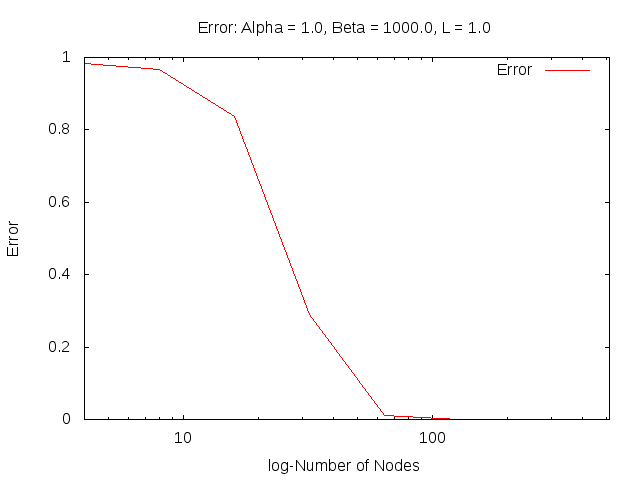
\includegraphics[scale = 0.5]{/home/john/Dropbox/C1/Assignment_4/Q3/Error_Plot_1_1000_1.png}}

In this graph we see that the approximate solution oscilliates around the exact solution. This can be explained by looking at the solution to the difference equation obtained from the finite difference approximation. By choosing large $\beta$ and small $\alpha$, $\Prob e_{gl}$ becomes large for fixed $h$. This causes the solution to the difference equation to oscillate due to the $(\frac{1 + \Prob e}{1 - \Prob e})^i$ term. We may prevent this by choosing a small step size $h$ however this is more computationally intensive. This can be seen from the second graph where the error only becomes small when a large number of nodes are used.

\end{document}
